\RequirePackage{fixltx2e} %This package in CTeX is not compatible with revtex4-1
\documentclass[aps,pre,12pt,preprint,onecolumn,showpacs,showkeys]{revtex4-1}
\usepackage{ctex}
\usepackage{mathtools,mathrsfs}
\usepackage{multirow}
\usepackage{setspace,dcolumn}
\usepackage{hyperref}
\usepackage{graphicx,psfrag,epsfig}
\usepackage[font=small,format=plain,labelfont=bf,textfont=it,justification=centering,singlelinecheck=false]{caption}
\usepackage{amsmath,amsfonts,amssymb,amsthm,bm,upgreek}
\usepackage{geometry}
\usepackage[mathscr]{eucal}
\usepackage{caption}
\usepackage{subcaption}
\hypersetup{colorlinks=true}
\geometry{top=2.54cm,bottom=2.54cm,left=3cm,right=3cm}
\renewcommand\appendixname{附录}
\renewcommand\abstractname{}%摘要
\renewcommand\tablename{表}
\renewcommand\figurename{图}
\makeatletter
\def\@pacs@name{\songti\zihao{-4}{\bf PACS码:}}
\def\@keys@name{\songti\zihao{-4}{\bf 关键词:}}
\def\Dated@name{日期:}
\def\Received@name{\zihao{-5}{接收} }
\def\Revised@name{\zihao{-5}{修订} }
\def\Accepted@name{\zihao{-5}{采纳} }
\def\Published@name{\zihao{-5}{发表} }
\makeatother
\linespread{1.3}
\renewcommand{\labelenumi}{\alph{enumi}.}
\leftmargini=20mm
\def \d {\mathrm d}
\def \degree {^\circ}
\def \V {\bm{V}}
\def \degC {^\circ \mathrm{C}}

\begin{document}
\title{\bf\heiti\zihao{3}体效应振荡器的工作特性和波导管的工作状态\vspace{15mm}}
\author{\fangsong\zihao{4}邵智轩\vspace{2mm}}
\affiliation{\songti\zihao{-4}学号:1400012141\vspace{2mm}}
\date{\today}
%\pacs{02.10.Yn, 33.15.Vb, 98.52.Cf, 78.47.dc}
\keywords{体效应振荡器,特性曲线,波导管,功率,频率,驻波比,微波元件}
\email{shaozhixuansh@pku.edu.cn; (86)13381350619}

\begin{abstract}
\vspace{10mm}
\begin{spacing}{1.5}
\songti\zihao{-4}
本实验目的为:了解体效应振荡器的结构、工作原理和工作特性及波导管的三种工作状态;掌握微波的三种基本参量的测量方法、测量波导波长$\lambda_g=48.90$ mm、确定波导管中波传播的相速度$v_g=4.401\times 10^8$ m/s,光速$c=3.005\times 10^8$ m/s,群速度$u=2.053\times 10^8$ m/s。

\end{spacing}
\end{abstract}
\maketitle
\songti\zihao{-4}

\section{引言}
微波是波长很短、频率很高的电磁波。由于它有一系列特殊的性质,因而在国防、通讯、工农业生产、科学研究以及日常生活中得到广泛的应用。了解微波的产生和传输特性,掌握有关微波的一些基本参量,如功率、频率、电压驻波比的测量原理和测量方法,对熟悉和掌握微波技术是必不可少的。

\section{实验原理}
    \subsection{体效应振荡器的结构和工作特性}
    将体效应二极管适当放置在高 $Q$ 谐振腔中,构成谐振电路,以便产生微波振荡。对于不同类型的体效应管应配以相应的谐振腔,使之达到较好的匹配,工作在渡越时间模式或者畴模式。本实验中的固态源采用机械调谐方式,频率由数字表直接显示。

    \begin{figure}[ht]
        \centering
        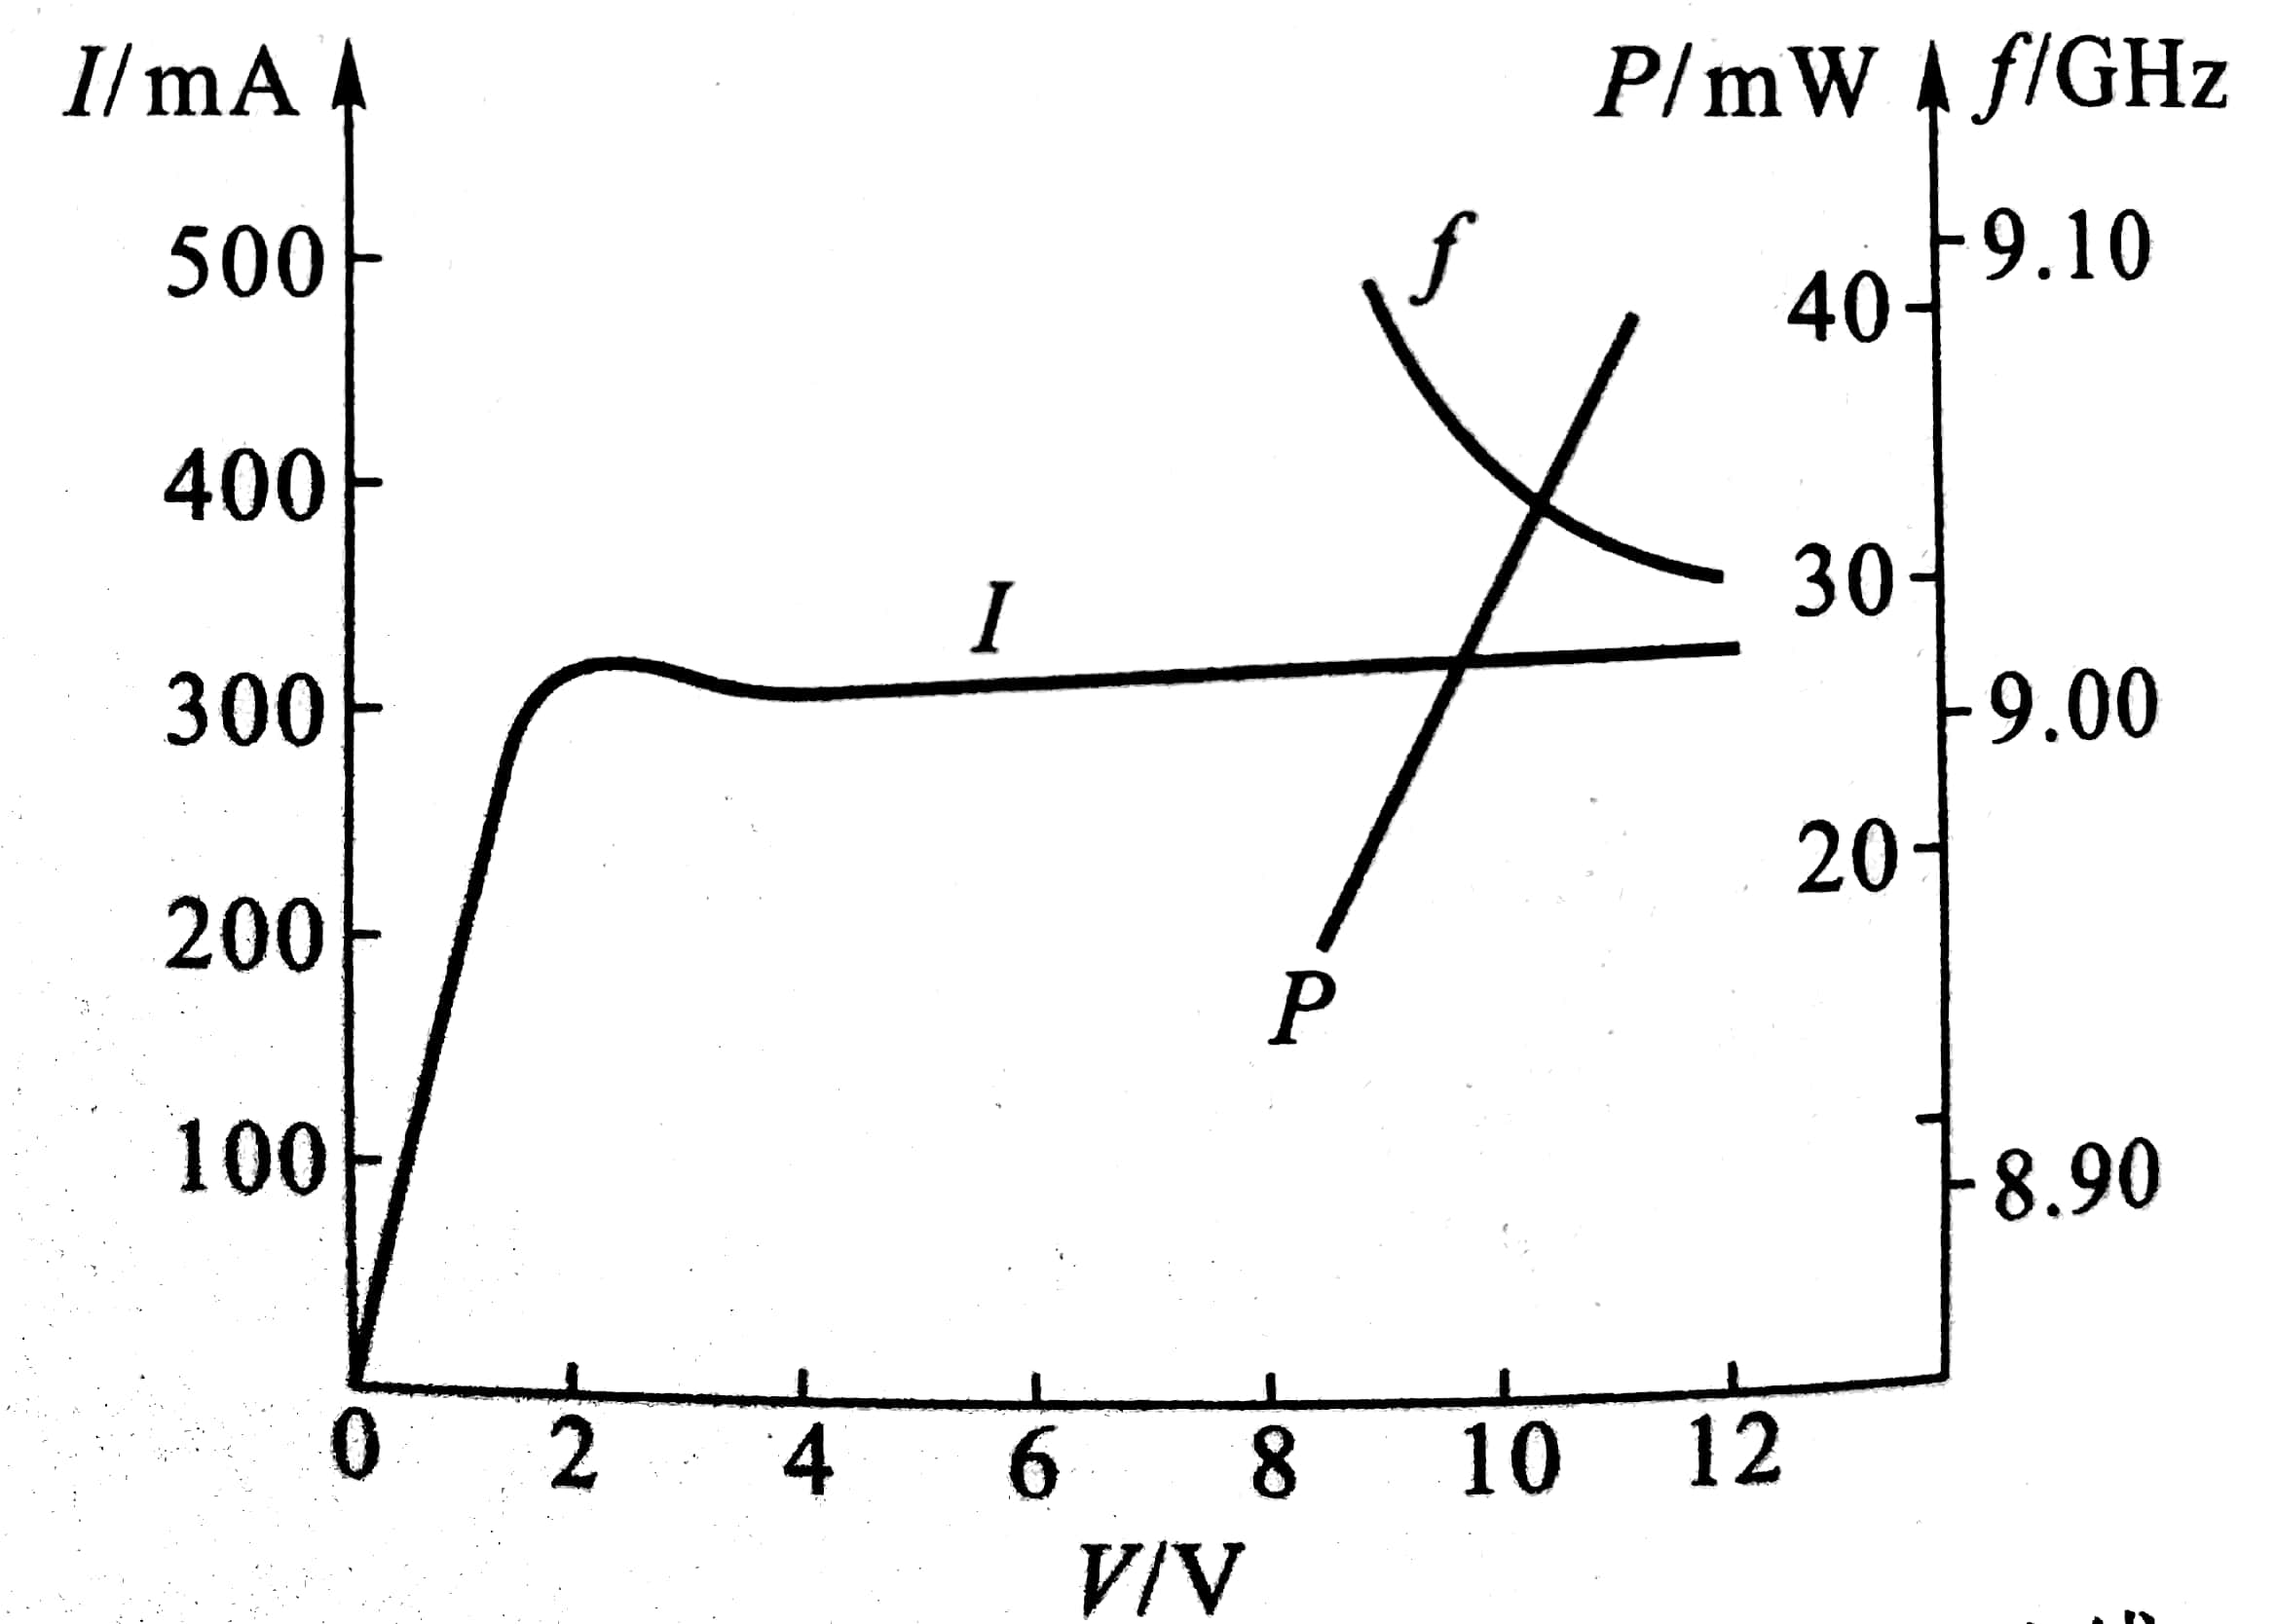
\includegraphics[width=100mm]{typical}
        \caption{\label{fig:typical}%
        体效应振荡器的典型特性曲线}
    \end{figure}

    体效应振荡器的一组典型特性曲线如图\ref{fig:typical}所示。使腔体的尺寸一定,改变体效应管的工作电压,其工作电流、微波输出功率和频率都将发生变化。在阈值电压以下,体效应管的电流随电压几乎线性增长,而当电压超过阈值时,由于偶极畴的产生和快速成长,电流下降,继续增加电压,电流变化平缓。这在畴形成向阳极渡越直至消失的过程中都是如此。此外,随工作电压的增加,输出功率增加,而振荡频率降低。当然,并非所有体效应振荡器的功率和频率与工作电压间的关系都类似图\ref{fig:typical}的形式。不同的体效应管由于半导体材料中掺杂、缺陷或位错等微观情况不完全一致,因而振荡器的工作特性一般来说是不相同的。

    \subsection{波导管的工作特性}
        \subsubsection{波导管中波的传播特性}
        一般来说,波导管中存在入射波和反射波。描述波导管中匹配和反射程度的物理量是驻波比或反射系数。由于终端情况不同,波导管中电磁场的分布情况也不同,可以把波导管的工作状态归结为三种状态:
        \begin{itemize}
            \item 匹配状态:不存在反射波,$|E|=|E_i|$;
            \item 驻波状态:终端发生全反射,$|E_i|=|E_r|$,所以在驻波波腹处$|E|_{\max}=|E_i|+|E_r|$,驻波波节处$|E|_{\min}=|E_i|-|E_r|=0$;
            \item 混波状态,终端是部分反射,$|E_r|<|E_i|$,所以$|E|_{\max}=|E_i|+|E_r|$, $|E|_{\min}=|E_i|-|E_r|\ne 0$。
        \end{itemize}

        波导管中的波导波长$\lambda_g$大于自由空间波长$\lambda$,由于
        \begin{equation}
            c=\lambda f
        \end{equation}
        \begin{equation}
            v_g=\lambda_g f
        \end{equation}
        式中$c$为光速,$v_g$为相速度。波导管中波传播的相速度$v_g$大于光速$c$。相速度只是相位变化的速度,并非波导管中波能量的传播速度(群速度$u$),因此相速度可以大于光速。相速度$v_g$、群速度$u$、光速$c$的关系式为:
        \begin{equation}
            v_g u = c^2
        \end{equation}
        
        实验中,我们通过测量波导波长$\lambda_g$和频率$f$来决定光速$c$、相速度$v_g$和群速度$u$。

        \subsubsection{驻波测量}
        检波晶体管的检波电流$I$与探针所在处的电场大小$E$满足关系式:
        \begin{equation}
            I=k_1 E^n
        \end{equation}
        在小功率情况下,可以相当精确地认为满足平方律检波,$n\approx 2$。

        小驻波比($1.005 \le \rho \le 1.5$)的测量:驻波波腹和波节都不尖锐,因此要多测几个驻波波腹和波节,按下式计算$\rho$的平均值:
        \begin{equation}
            \rho =\frac{E_{\max\,1}+E_{\max\,2}+...+E_{\max\,n}}{E_{\min\,1}+E_{\min\,2}+...+E_{\min\,n}}
        \end{equation}
        当检波晶体满足平方律时,
        \begin{equation}
            \rho =\frac{\sqrt{I_{\max\,1}}+\sqrt{I_{\max\,2}}+...+\sqrt{I_{\max\,n}}}{\sqrt{I_{\min\,1}}+\sqrt{I_{\min\,2}}+...+\sqrt{I_{\min\,n}}}
        \end{equation}

        中驻波比($1.5\le \rho \le 10$)的测量:此时只需测一个驻波波腹和一个波节,按下式计算:
        \begin{equation}
            \rho = \frac{E_{\max}}{E_{\min}}=\sqrt{\frac{I_{\max}}{I_{\min}}}
        \end{equation}
        
        \subsubsection{晶体检波特性曲线和检波律的测定}
        令驻波测量线终端短路(驻波状态),此时沿线个点驻波振幅与终端距离$l$的关系为:
        \begin{equation}
            |E|=k_2 \left|\sin \frac{2 \pi l}{\lambda_ g}\right|\label{eq:E-l}
        \end{equation}
        设以线上$l=l_0$处的驻波波节为参考点,将探针向某一边移动,每一处驻波电场值便有一相应的检波电流值。如果测量时不必知道检波律$n$,我们由实验测得$I(l)$,由式(\ref{eq:E-l})算出$|E(l)|$,直接画出$I-|E|$关系曲线,利用它可以实际测得的检波电流值找出相应的驻波电场相对值,从而求出正确的驻波比。

        如果需要直到检波律$n$,可以由实验测量在两个相邻波节之间的驻波曲线$I(l)$,再利用下列关系式定出$n$:
        \begin{equation}
            n=\frac{-0.3010}{\lg \cos\frac{\pi \Delta l}{\lambda _g}}\label{eq:n}
        \end{equation}
        其中$\Delta l$为驻波曲线上$I=I_m/2$两点的距离,$I_m$为波腹的检波电流。

\section{实验装置}
\begin{figure}[ht]
    \centering
    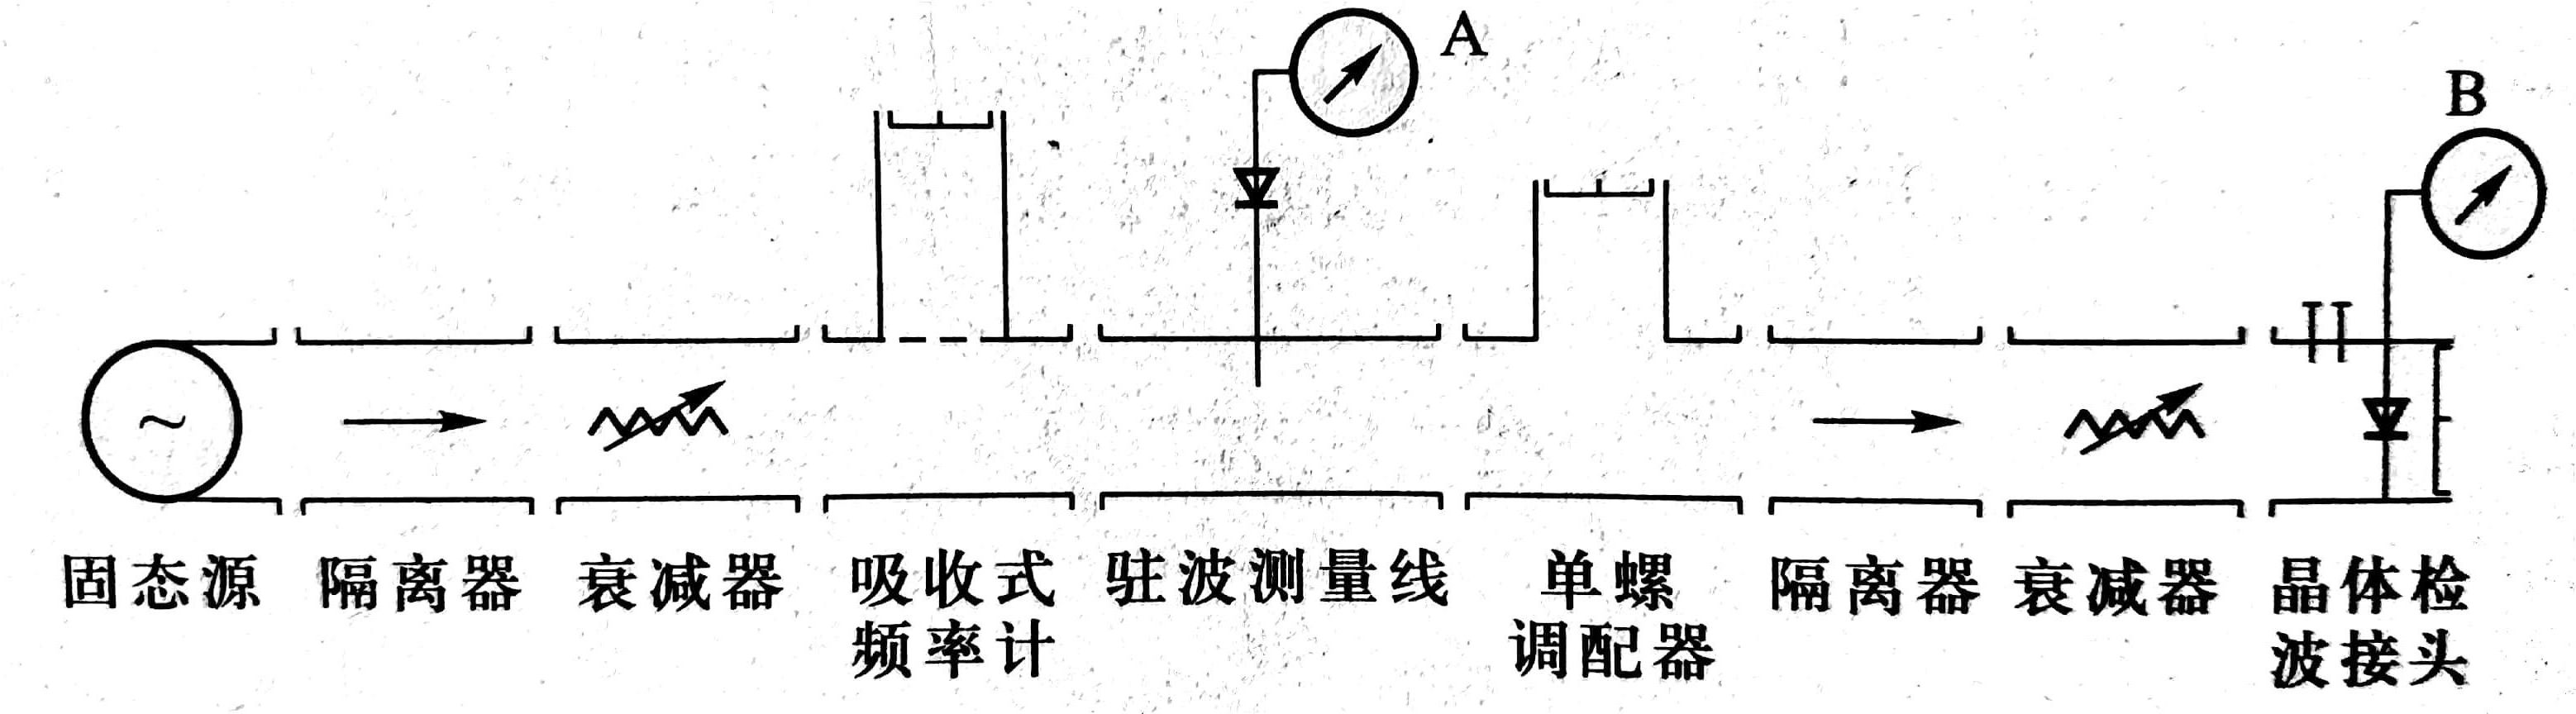
\includegraphics[width=120mm]{equip}
    \caption{\label{fig:equip}%
    实验线路}
\end{figure}

本实验采用的实验线路如图\ref{fig:equip}所示。

\section{实验内容}
    \subsection{测量体效应振荡器的工作特性曲线}
    将信号源的工作方式置于“等幅”状态,保持频率读数为 9.000 GHz 不变,通过电压调节钮,在 0 - 13.0 V 范围内连续改变体效应管的工作电压,并得到相应的工作电流显示。同时,通过测量装置中的波长表和光点检流计 B,测出频率和相对功率。测量数据如表\ref{tab:feature_curve}所示,工作特性曲线如图\ref{fig:feature_curve}所示。

    \begin{table}[h]
        \caption{\label{tab:feature_curve}%
        体效应振荡管的工作电流$I$、相对输出功率$P$、频率$f$随工作电压$V$的变化关系\footnote{当工作电压较小时,无法测量相对输出功率$P$和频率$f$,只测量工作电流$I$}}
        \begin{tabular}{|l|l|l|l|l|l|l|l|l|l|l|l|l|}
            \hline
            工作电压$V/$V&13.00&12.50&12.00&11.50&11.00&10.50&10.00&9.50&9.00&8.50&8.00&7.50\\\hline
            工作电流$I/$mA&352&308&306&306&306&306&306&306&307&308&309&311\\\hline
            相对输出功率$P$&95.5&87.4&80.2&74.9&63.2&52.4&39.0&28.0&18.5&11.5&6.2&2.0\\\hline
            波长表读数$\lambda/$cm&7.725&7.734&7.748&7.780&7.822&7.871&7.946&8.042&8.143&8.238&8.332&8.508\\\hline
            对应频率$f/$GHz&8.995&8.994&8.992&8.989&8.985&8.980&8.973&8.963&8.953&8.943&8.934&8.917\\\hline
        \end{tabular}
        \begin{tabular}{|l|l|l|l|l|l|l|l|l|l|l|l|}
            \hline
            工作电压$V/$V&7.00&6.50&6.00&5.50&5.00&4.50&4.00&3.80&3.50&3.40&3.20\\\hline
            工作电流$I/$mA&312&312&314&325&325&325&325&329&360&359&355\\\hline
        \end{tabular}
        \begin{tabular}{|l|l|l|l|l|l|l|l|l|l|l|l|}
            \hline
            工作电压$V/$V&3.00&2.70&2.50&2.30&2.10&1.80&1.50&1.20&0.90&0.60&0.30\\\hline
            工作电流$I/$mA&350&336&323&308&289&258&224&186&145&99&52\\\hline
        \end{tabular}
    \end{table}

    与教材给出的典型特性曲线(图\ref{fig:typical})相比,工作电流曲线的特点是基本吻合的,而频率$f$和工作电压$V$的关系与图\ref{fig:typical}的变化趋势完全相反。在实测的曲线中,在阈值电压以上,频率反而随电压增大而增加。这正说明了,由于不同的体效应管由于半导体材料中掺杂、缺陷或位错等微观情况不完全一致,因而振荡器的工作特性一般来说是不相同的。

    \begin{figure}[ht]
        \centering
        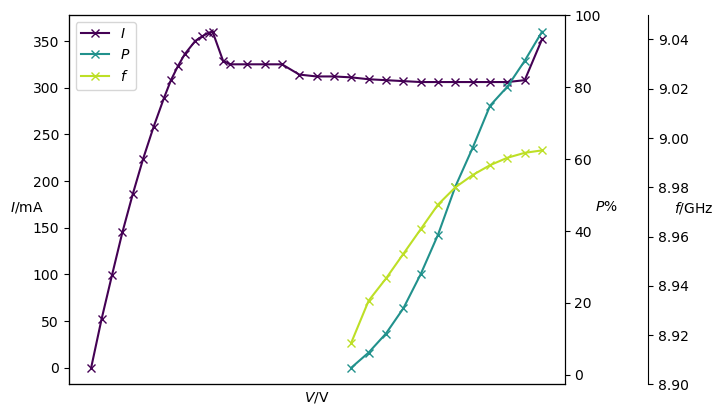
\includegraphics[width=120mm]{feature_curve}
        \caption{\label{fig:feature_curve}%
        实验测得的体效应振荡管的特性曲线}
    \end{figure}

    \subsection{观测波导管的工作状态}
        \subsubsection{测量小驻波比与中驻波比}
        在“等幅”状态下,频率显示为 9.000 GHz,体效应管的工作电压为 12.02 V。
        
        利用单螺调配器改变测量线终端的状态,可调制最佳匹配状态($\rho<1.10$),此时实测的小驻波比为:
        \begin{equation}
            \rho=\frac{\sqrt{59.8}+\sqrt{59.5}+\sqrt{59.1}+\sqrt{58.0}}{\sqrt{51.5}+\sqrt{51.5}+\sqrt{51.4}+\sqrt{51.0}}=1.07
        \end{equation}
        反射系数:
        \begin{equation}
            |\Gamma_0|=\frac{\rho-1}{\rho+1}=0.034
        \end{equation}

        利用单螺调配器改变测量线终端的状态,可调制最佳混波状态($2<\rho<3$),此时实测的中驻波比为:
        \begin{equation}
            \rho=\sqrt{\frac{93}{23}}=2.01,\quad |\Gamma_0|=\frac{\rho-1}{\rho+1}=0.336
        \end{equation}
    
        \subsection{测量波导波长}
        相邻两个波节间的距离即为波导波长$\lambda_g$的一半,实测结果为
        \begin{equation}
            \lambda_g=48.90 \mathrm{mm}
        \end{equation}
        则群速度$v_g=\lambda_g f=4.401\times 10^8$ m/s。已知波导管宽边$a=22.86$ mm,自由空间波长
        \begin{equation}
            \lambda=\frac{\lambda_g}{\sqrt{1+\left(\frac{\lambda_g}{2a}\right)^2}}=33.40 \mathrm{mm}
        \end{equation}
        由此可计算光速$c$和群速度$u$:
        \begin{equation}
            c=\lambda f=3.005\times 10^8 \mathrm{m/s}
        \end{equation}
        \begin{equation}
            u=\frac{c^2}{v_g}=2.053\times 10^8 \mathrm{m/s}
        \end{equation}

        \subsubsection{测量两个相邻波节之间的驻波曲线$I(l)$,作出检波晶体管的$I-|E|$曲线,确定晶体检波律$n$}
        在不同位置$l$处记录检波电流$I$的大小,数据如表\ref{tab:I_l}所示,$I(l)$曲线如图\ref{fig:I_l}所示,$I-|E|$曲线如图\ref{fig:I_E}所示。
        \begin{table}[h]
            \caption{\label{tab:I_l}%
            两个相邻波节之间的检波电流$I$随位置$l$的变化关系}
            \begin{tabular}{|l|l|l|l|l|l|l|l|l|l|}
                \hline
                实际位置$x$/mm&146.7&142.8&\textbf{140.6}&138.2&133.8&129.6&\textbf{128.0}&126.6&121.9\\\hline
                相对位置$l$/mm&0&3.9&6.1&8.5&12.9&17.1&18.7&20.1&24.8\\\hline
                检波电流$I$/mA&2.0&30.0&58.5&93.0&119.0&83.0&58.5&37.0&2.2\\\hline
            \end{tabular}
        \end{table}

        \begin{figure}[ht]
            \begin{minipage}{.5\textwidth}
                \centering
                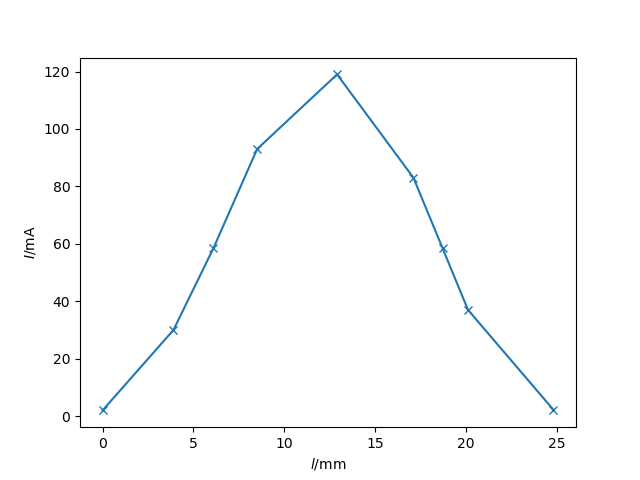
\includegraphics[width=85mm]{I_l}
                \caption{\label{fig:I_l}%
                实测$I-l$曲线}
            \end{minipage}%
            \begin{minipage}{0.5\textwidth}
                \centering
                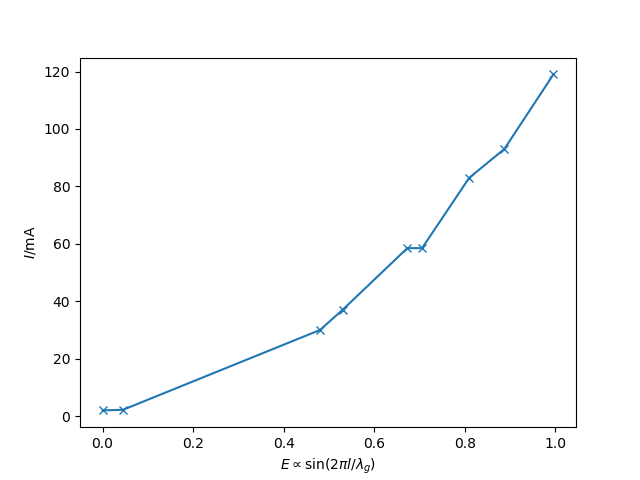
\includegraphics[width=85mm]{I_E}
                \caption{\label{fig:I_E}%
                实测$I-|E|$曲线}
            \end{minipage}
        \end{figure}

        将实测的半高宽$\Delta l$代入式(\ref{eq:n})得
        \begin{equation}
            n=\frac{-0.3010}{\lg \cos\frac{\pi (18.7-6.1)}{48.9}}=1.87
        \end{equation}

\section{致谢}
感谢王常生老师对实验的悉心指导,使我自己摸索出了微波元器件的使用方法及波导管的工作特性,最终克服困难,顺利完成实验。尤其是王老师主张让我们自己多琢磨琢磨,要敢于尝试,勤于思考,这种精神让我受益匪浅。
    
\begin{thebibliography}{}
\bibitem{Book} 吴思诚, 荀坤. 近代物理实验(第四版). 北京:高等教育出版社, 2015
\end{thebibliography}
\end{document}